\documentclass[14pt]{extarticle}%
\usepackage{textcomp}%
\usepackage{lastpage}%
\usepackage[russian]{babel}%
\usepackage{titling}%
\usepackage{nopageno}%
\usepackage{amssymb}%
\usepackage{amsmath}%
\usepackage{tabto}%
\usepackage[left=3cm,right=1cm, top=2cm,bottom=2cm]{geometry}%
\usepackage{circuitikz}%

%
\title{Задача о расположении сенсоров для мультиграфа}%
\DeclareMathOperator*{\amper}{\&}%
\date{}%
%
\begin{document}%
\normalsize%
\vspace{-80pt}%
\begin{center}
    \textbf{Введение}
\end{center}

Будем рассматривать разреженные линейные недоопределенные системы с вложенной сетевой структурой. Их структура наследуется из задач где применяются неоднородные сетевые потоки с переменными внешними потоками узлов. Одно из приложений рассматриваемых недоопределенных систем --- задача о расположении сенсоров для мультиграфа. Задача заключается в расположении минимального количества сенсоров в узлах мультиграфа для определения величины потока на дугах и переменных интенсивностей узлов для всего мультиграфа. Исследование ранга разреженной матрицы основано на конструктивной теории декомпозиции разреженных СЛАУ.

Данная задача имеет широкое практическое применение, пример которого будет рассмотрен далее.

Для реализации алгоритмов, описанных в работе используется система компьютерной алгебры Wolfram Mathematica. Данная система компьютерной алгебры включает в себя возможность производить символьные вычисления, что позволяет построить общее решение для рассматриваемой разреженной СЛАУ и, используя возможности системы по упрощению логических выражений, проверить и продемонстрировать корректность построенного общего решения, а также наглядно продемонстрировать построенные вспомогательные структуры. Более того, данная система компьютерной алгебры предоставляет широкие возможности по оптимизации кода, такие как автоматическая параллелизация вычислений и компиляция часто используемых модулей, что позволяет значительно увеличить скорость вычислений.


\newpage
\begin{center}
    \textbf{Глава 1. ТЕОРЕТИЧЕСКАЯ ОСНОВА И ПОСТАНОВКА ЗАДАЧИ}
\end{center}

Пусть $G=(I,U)$ --- конечный ориентированный связный мультиграф без циклов с множеством узлов $I$ и множеством дуг $U$, $|U|>>|I|$. Пусть \\$K (|K|~<~\infty)$ --- множество различных потоков, проходящих через сеть $G$. Полагаем $K=~\{1,\dots,~|K|\}$. Зафиксируем связную сеть, соответствующую конкретному потоку $k\in K$: $G^k=(I^k, U^k), I^k\subseteq I,U^k=\{(i,j)^k:(i,j)\in \widehat{U}^k\}$,$\widehat{U}^k\in U$ --- множество дуг $G$, по которым проходит поток $k\in K$. Кроме того, для каждой мультидуги $(i,j)\in U$ введем множество $K(i,j)=\{k\in K:(i,j)^k\in U^k\}$, которое содержит все потоки, проходящие по мультидуге $(i,j)$.

\textbf{1.1 Построение СЛАУ для рассматриеваемого мультиграфа}

Рассмотрим сладующую разреженную недоопределенную СЛАУ:

\begin{equation}
 \sum_{j\in I^+_i(U^k)} x^k_{ij}-\sum_{j\in I^-_i(U^k)}x^k_{ji}=\left\{\begin{matrix}
a^k_i, & i\in I^k\setminus I^*_k,\\ 
x^k_i sign(i), & i\in I^*_k.
\end{matrix}\right., k\in K,\label{f1}   
\end{equation}
 \begin{equation}
     \sum_{k\in K}\left(\sum_{(i,j)^k\in U^k}\lambda^{k,p}_{ij}x^k_{ij}\right)+\sum_{k\in K}\sum_{i\in I^*_k}\lambda^{k,p}_ix^k_i=\beta_p, p=\overline{1,q}. \label{f2}
 \end{equation}
 
Здесь $I^+_i(U^k)=\{j\in I^k:(i,j)^k\in U^k\}, I^-_i(U^k)=\{j\in I^k:(j,i)^k\in U^k\}$, $x^k_{ij}$ --- величина потока вдоль дуги $(i,j)^k$. Узлы $i^k\in I^*_k, k\in K$ (обозначаем $i$ если $k$ определено контекстом) называются динамическими (или базисными) --- узлы с переменной интенсивностью $x^k_i$,\\
$$sign(i^k)=\left\{
\begin{matrix}
1,  & i^k\in I^*_{k+},\\
-1, & i^k\in I^*_{k-};
\end{matrix}
\right.$$
$$I^*_{k+}, I^*_{k-}\subseteq I^*_k, I^*_{k+} \cap I^*_{k-}=\varnothing$$,
$$a^k_i, \lambda^{k,p}_{ij}, \lambda^{k,p}_i, \beta_p\in \mathbb{R}$$

Матрица системы (\ref{f1}) - (\ref{f2}) имеет блочную структуру вида:
$$A=\left[\begin{matrix}
M&B\\
Q&T
\end{matrix}\right]$$

Здесь $M$ --- матрица с блочно-диагональной структурой размера \\$\sum_{k\in K}|I^k|\times~\sum_{k\in K}|U^k|$, т.к. каждый ее блок представляет из себя матрицу размера $|I^k|\times|U^k|$ --- матрицу инцидентности сети $G^k=(I^k,U^k), k\in K$, условно запишем $M=M_1\bigoplus\dots\bigoplus M_{|K|}$, где $M_k, k\in K$ --- блоки матрицы $M$; $Q$ --- матрица размера $q\times\sum_{k\in K}|U^k|$ с элементами $\lambda^{k,p}_{ij}, (i,j)\in U, k\in K(i,j), p=\overline{1,q}$. Матрица $B$ --- разреженная матрица с блочно-диагональной структурой размера $\sum_{k\in K}|I^k|\times \sum_{k\in K}|I^*_k|$, т.к. каждый ее блок представляет из себя матрицу размера $|I^k|\times|I^*_k|$ матрицы сети $G^k, k\in K$, условно запишем $B=B_1\bigoplus\dots\bigoplus B_{|K|}$. Матрица $B_k$ колонке $j$ имеет ненулевой элемент равный $-sign(i)$ в строоке $i$ для всех $j\in I^*_k$, все остальные элементы равны нулю, $i\in I^k, k\in K$. $T$ --- матрица размера $q\times\sum_{k\in K}|I^*_k|$ и состоит из элементов $\lambda^{k,p}_i, i\in I^*_k, k\in K, p=\overline{1,q}$. В [1], [3] рассмативаются СЛАУ с включенной сетевой структурой. Их структура унаследована из задач о гомогенном сетевом потоке с узлами с переменным внешним потоком. В [4] исследуются разреженные линейные системы с фрактальными матрицами. В этой работе рассматривается алгоритм декомпозиции разреженных систем для мультиграфа, которые используются в задаче расположения сенсоров.

Считаем, что $\sum_{k\in K}|I^k|+q<\sum_{k\in K}|U^k|+\sum_{k\in K}|I^*_k|$.

\textbf{Теорема 1.} \textit{Ранг матрицы $[M_k \ B_k]$ cистемы (\ref{f1}) для фиксированного $k\in K$ и графа $G^k, I^*_k\neq\varnothing$ равен $|I^k|$[1].}

Характеристический вектор цикла, характеристический вектор цепи с учетом направления с привязкой к узлу, характеристический вектор цепи с учетом направления с привязкой к дуге для заданного $k\in K$ составлены в соответствии с правилами [1].

\textbf{Теорема 2.} \textit{Характеристический вектор цикла, характеристический вектор цепи с учетом направления с привязкой к узлу, характеристический вектор цепи с учетом направления с привязкой к дуге для заданного $k\in K$ удовлетворяют системе (\ref{f3})[1,2].}
\begin{equation}
     \sum_{j\in I^+_i(U^k)} x^k_{ij}-\sum_{j\in I^-_i(U^k)}x^k_{ji}=\left\{\begin{matrix}
0, & i\in I^k\setminus I^*_k,\\ 
x^k_i sign(i), & i\in I^*_k.
\end{matrix}\right., k\in K.\label{f3} 
\end{equation}\\

\textbf{Теорема 3.} \textit{Любое решение системы 3 для фиксированного $k\in K$ есть линейная комбинация характеристических векторов [1].}

О п р е д е л е н и е 1. {\itБудем называть упорядоченную пару множеств \\$R=\{U^k_R, I^{*k}_R, k\in K\}, U^k_R\subseteq U^k$ и $I^{*k}_R\subseteq I^*_k$ опорой для мультиграфа $G$ и системы (\ref{f1}) если для него система 
\begin{equation}
     \sum_{j\in I^+_i(\widetilde U^k)} x^k_{ij}-\sum_{j\in I^-_i(\widetilde U^k)}x^k_{ji}=\left\{\begin{matrix}
0, & i\in I^k\setminus \widetilde I^*_k,\\ 
x^k_i sign(i), & i\in \widetilde I^*_k.
\end{matrix}\right., k\in K.\label{f4} 
\end{equation}\\
при $U^k=U^k_R, I^*_k=I^{*k}_R$ имеет единственное тривиальное решение, но при этом для всех следующих пар множеств система (\ref{f4}) имеет нетривиальные решения:\\

$\widetilde R=\{\widetilde{U}^k, \widetilde{I}^*_k, k\in K\},$

$\widetilde{U}^{k_0}=U^{k_0}_R\cup(i_0,j_0)^{k_0}, (i_0,j_0)^{k_0}\in (U^{k_0}\setminus U^{k_0}_R);$

$\widetilde{U}^k=U^k_R, k\in (K\setminus k_0); \widetilde{I}^*_k=I^{*k}_R, k\in K$

$\widetilde R=\{\widetilde{U}^k, \widetilde{I}^*_k, k\in K\},$

$\widetilde{U}^k=U^k_R, k\in K; \widetilde{I}^*_{k_0}=(I^{*k_0}_R\cup \{i_0\}), i_0\in (I^*_{k_0}\setminus I^{*k_0}_R); \widetilde{I}^*_{k}=I^{*k}_R, k\in (K\setminus k_0).
$}

Для подмножества дуг $U_1\subseteq U$ введем понятие множества ницедентных узлов как $$I(U_1)=\{i\in I: (i,j)\in~U_1\vee (j,i)\in U_1\}.$$

Для каждого $k\in K$ построим лес из $\widetilde t_k$ деревьев $T^{k,t_k}=\{I^{k,t_k}_T, U^{k,t_k}_T\}$, где $I^{k,t_k}_T=I\left(U^{k,t_k}_T\right), U^{k,t_k}_T\subseteq U^k_R,\\ t_k=~\overline{1,\widetilde t_k}$, таких, что каждое дерево $T^{k,t_k}$ содержит ровно один узел \\$u_{t_k}\in I^{*k}_R, \,\forall t_k=\overline{1,\widetilde t_k},\, k\in K$.

Для каждого $k\in K$ построим следующие множества:
$$U^k_R=\bigcup_{t_k=1}^{\widetilde t_k}U^{k,t_k}_T,\,\,I^{*k}_R=\left\{u_{t_k}:t_k=\overline{1,\widetilde t_k}\right\}$$

\textbf{Теорема 4.} {\it(Критерий опоры сети)\\
Упорядоченная пара множеств $R=\{U^k_R, I^{*k}_R, k\in K\},U^k_R\subseteq U^k, I^{*k}_R\subseteq I^*_k$ является опорой мультиграфа $G$ для системы (\ref{f1}) тогда и только тогда, когда выполняются следуюшие условия:
\begin{enumerate}
\item Каждая компонента связности $T^{k,t_k}=\{I(U^{k,t_k}_T), U^{k,t_k}_T\}, t_k=\overline{1,\widetilde t_k}$ является деревом;

\item Множество узлов леса $T^{k,t_k}=\{I(U^{k,t_k}_T), U^{k,t_k}_T\}, t_k=\overline{1,\widetilde t_k}$ покрывает все узлы графа $G^k=(I^k, U^k)$, то есть выполняется:
$$\bigcup_{t_k=1}^{\widetilde t_k} I\left(U^{k,t_k}_T\right)=I^k;$$


\item Каждая компонента связности $T^{k,t_k}=\{I(U^{k,t_k}_T), U^{k,t_k}_T\}, t_k=\overline{1,\widetilde t_k}$ содержит ровно один базисный узел из $I^{*k}_R$, то есть выполняется:
$$|I^{*k}_R\cap I\left(U^{k,t_k}_T\right)|=1,\, \forall t_k=\overline{1,\widetilde t_k}.$$
\end{enumerate}}

После того, как опора $R=\{U^k_R, I^{*k}_R, k\in K\}$ мультиграфа $G$ для системы (\ref{f1}) построена, можно рассмотреть несколько структур, которые могут быть получены путем добавления одной неопорной дуги к опоре $R$.

О п р е д е л е н и е 2. {\it Характеристическим вектором, порожденным дугой $(\tau, \rho)^k\in \left(U^k\setminus U^k_R\right)$ называется вектор 
$$\delta^k(\tau,\rho)=(\delta^k_{ij}(\tau, \rho), (i,j)^k\in U^k; \delta^k_i(\tau, \rho), i\in I^*_k),$$ 
построенный по следующим правилам для фиксированного $k$:

1)  Если множество $U^k_R\cup\{(\tau, \rho)^k\}$ имеет цикл $L_k=\{I^k_L, U^k_L\}$, то $\delta^k(\tau, \rho)$ --- характеристический вектор этого цикла и дуга $(\tau, \rho)^k$ выбирается как оперделяющая направление обхода цикла.

2)  Если в множестве $U^k_R\cup\{(\tau, \rho)^k\}$ содержится цепь $C_k={I^k_C, U^k_c}$, соединяющая узлы $u$ и $v\, \in I^{*k}_R$, то $\delta^k(\tau, \rho)$~--- характеристический вектор цепи и дуга $(\tau, \rho)^k$ выбирается как оперделяющая направление обхода цепи $C$.}

О п р е д е л е н и е 3.  \textit{Характеристическим вектором, порожденным узлом $\gamma\in (I^k\setminus I^{*k}_R)$ называется вектор 
$$\delta^k(\gamma)=(\delta^k_{ij}(\gamma), (i,j)^k\in U^k; \delta^k_i(\gamma), i\in I^*_k),$$
 построенный как характеристический вектор цепи для фиксированного $k$, которая соединяет узлы $\gamma$ и $v\in I^{*k}_R$, причем направление цепи выбирается таким образом, что $\gamma$~---~ее начало.}

    \textbf{Теорема 5.}  {\itОбщее решение системы (\ref{f1}) для фиксированного $k\in K$ может быть представлено в виде:
    \begin{equation}
        x^k_{ij}=\sum_{(\tau, \rho)^k\in (U^k\setminus U^k_R)}x^k_{\tau \rho}\delta^k_{ij}(\tau,\rho)+\sum_{\gamma\in I^*_k\setminus I^{*k}_R}x^k_\gamma\delta^k_{ij}(\gamma)+\widetilde x^k_{ij},\,\,\,\, (i,j)^k\in U^k_R;\label{f5}\end{equation}
    \\
    \begin{equation}
        x^k_i=\sum_{(\tau, \rho)^k\in (U^k\setminus U^k_R)}x^k_{\tau \rho}\delta^k_{i}(\tau,\rho)+\sum_{\gamma\in I^*_k\setminus I^{*k}_R}x^k_\gamma\delta^k_{i}(\gamma)+\widetilde x^k_{i},\,\,\,\, i\in I^{*k}_R;\label{f6}\end{equation}
        \\
        где $\widetilde x^k=(\widetilde x^k_{ij}, (i,j)\in U^k;\; \widetilde x^k_i, i\in I^*_k)$ --- частное решение неоднородной системы (\ref{f1}), то есть вектор $(x^{*k}_{ij},x^{*k}_i)$ определенный как:
        
        $$
        x^{*k}_{ij}=\sum_{(\tau, \rho)^k\in (U^k\setminus U^k_R)}x^k_{\tau \rho}\delta^k_{ij}(\tau,\rho)+\sum_{\gamma\in I^*_k\setminus I^{*k}_R}x^k_\gamma\delta^k_{ij}(\gamma),\,\,\,\, (i,j)^k\in U^k_R;$$
    \\
    $$
        x^{*k}_i=\sum_{(\tau, \rho)^k\in (U^k\setminus U^k_R)}x^k_{\tau \rho}\delta^k_{i}(\tau,\rho)+\sum_{\gamma\in I^*_k\setminus I^{*k}_R}x^k_\gamma\delta^k_{i}(\gamma),\,\,\,\, i\in I^{*k}_R;$$
    является решением однородной системы (\ref{f3}).}

Доказательство этой теоремы для фиксированного $k$ можно найти в [1,3], общее неоднородное решение системы (\ref{f1}) назходится как сумма общего решения однородной системы (\ref{f3}) и любого частного решения неоднородной системы (\ref{f1}).

Заметим, что теорема 5 и формулы (\ref{f5})-(\ref{f6}) справедливы для любого частного решения $\widetilde x^k=(\widetilde x^k_{ij}, (i,j)\in~U^k; \widetilde x^k_i, i\in~I^*_k)$ системы (\ref{f1}), таким образом можно наложить ограничение на это частное решение, например, положить:

$$\widetilde x^k_{\tau\rho}=0, (\tau,\rho)\in U^k\setminus U^k_R;$$
$$ \widetilde x^k_\gamma=0, \gamma\in I^*_k\setminus I^{*k}_R$$


Далее будем использовать формулы (\ref{f5})-(\ref{f6}), подразумевая, что частное решение $\widetilde x^k$ построено в соответствии со введенными ограничениями.

 \textbf{1.2 Опора мультиграфа для системы дополнительных уравнений}

Пусть $R=\{U^k_R, I^{*k}_R, k\in K\},U^k_R\subseteq U^k, I^{*k}_R\subseteq I^*_k$ --- опора мультиграфа $G$ для системы (\ref{f1}). Выберем произвольно множества $W=\{U^k_W, I^{*k}_W, k\in K\},$\\ $|W|=q, U^k_W\subseteq U^k\setminus U^k_R, I^{*k}_W\subseteq I^*_k\setminus I^{*k}_R$. Если подставить общее решение системы (\ref{f1}), которое имеет вид (\ref{f5})-(\ref{f6}) в систему (\ref{f2}), система (\ref{f2}) примет следующий вид:

\begin{equation}
     \sum_{k\in K}\left(\sum_{(\tau,\rho)^k\in U^k\setminus U^k_R}\Lambda^{k,p}_{\tau\rho}x^k_{\tau\rho}\right)+\sum_{k\in K}\left(\sum_{\gamma\in I^*_k\setminus I^{*k}_R}\Lambda^{k,p}_\gamma x^k_\gamma\right)=A_p, p=\overline{1,q}, \label{f7}
 \end{equation}
 где
 $$
 \Lambda^{k,p}_{\tau\rho}=\lambda^{k,p}_{\tau\rho}+\sum_{(i,j)^k\in U^k_R}\lambda^{k,p}_{ij}\delta^k_{ij}(\tau, \rho)+\sum_{i\in I^{*k}_R}\lambda^{k,p}_{i}\delta^k_{i}(\tau, \rho),
 $$
 $$
 \Lambda^{k,p}_{\gamma}=\lambda^{k,p}_{\gamma}+\sum_{(i,j)^k\in U^k_R}\lambda^{k,p}_{ij}\delta^k_{ij}(\gamma)+\sum_{i\in I^{*k}_R}\lambda^{k,p}_{i}\delta^k_{i}(\gamma),
 $$
 $$
 A_p=\beta_p-\sum_{k\in K}\sum_{(i,j)^k\in U^k_R}\lambda^{k,p}_{ij}\widetilde x^k_{ij}-\sum_{k\in K}\sum_{i\in I^{*k}_R}\lambda^{k,p}_{i}\widetilde x^k_{i}.
 $$
 
 В системе (\ref{f7}) отделим переменные, относящиеся ко множеству $W$, после чего получим (\ref{f8})
 \begin{equation}
     \sum_{k\in K}\sum_{(\tau,\rho)^k\in U^k_W}\Lambda^{k,p}_{\tau\rho}x^k_{\tau\rho}+\sum_{k\in K}\sum_{\gamma\in I^{*k}_W}\Lambda^{k,p}_\gamma x^k_\gamma=A_p- \sum_{k\in K}\sum_{(\tau,\rho)^k\in U^k\setminus(U^k_W\cup U^k_R)}\Lambda^{k,p}_{\tau\rho}x^k_{\tau\rho}-\label{f8}
 \end{equation}
 
 $$-\sum_{k\in K}\sum_{\gamma\in I^*_k\setminus(I^{*k}_W\cup I^{*k}_R)}\Lambda^{k,p}_\gamma x^k_\gamma,\; p=\overline{1,q}$$

\textbf{1.3 Теоретические свойства мультиграфов}


О п р е д е л е н и е 4.  Будем называть опорой мультиграфа $G$ для систем (\ref{f1})-(\ref{f2}) такую упорядоченную пару множеств \\$Z=\{U^k_Z, I^{*k}_Z, k\in K\}, U^k_Z\subseteq U^k,\, I^{*k}_Z\subseteq I^*_k$, что для $\widetilde Z= \{\widetilde U^k,\widetilde I^*_k, k\in K\}$, при $\widetilde U^k=U^k_Z, \widetilde I^*_k=I^{*k}_Z$ система

\begin{equation}
\begin{gathered}
\sum_{j\in I^+_i(\widetilde U^k)} x^k_{ij}-\sum_{j\in I^-_i(\widetilde U^k)}x^k_{ji}=\left\{\begin{matrix}
0, & i\in I^k\setminus \widetilde I^*_k,\\ 
x^k_i sign(i), & i\in \widetilde I^*_k;
\end{matrix}\right.,\; k\in K;\\ \\
\sum_{k\in K}\left(\sum_{(i,j)^k\in\widetilde U^k}\lambda^{k,p}_{ij}x^k_{ij}\right)+\sum_{k\in K}\sum_{i\in\widetilde I^*_k}\lambda^{k,p}_ix^k_i=0,\; p=\overline{1,q} 
\end{gathered}\label{f9}
\end{equation}\\
имеет только тривиальное решение, но система (\ref{f9}) имеет нетривиальное решение хотя бы для одной из следующих пар $\widetilde Z$:
\begin{enumerate}
    \item 
    $\>\widetilde Z= \{\widetilde U^k,\widetilde I^*_k, k\in K\}$, при $\widetilde U^{k_0}=U^{k_0}_Z\cup \{(i_0, j_0)^{k_0}\}, (i_0, j_0)^{k_0}\in U^{k_0}\setminus U^{k_0}_Z;$\\
    $\widetilde U^k=U^k_Z$, при $k\in K\setminus \{k_0\};$\\
    $\widetilde I^*_k=I^{*k}_Z,\; k\in K;$
    \item $\>\widetilde Z= \{\widetilde U^k,\widetilde I^*_k, k\in K\}$ при $\widetilde U^k=U^k_Z$, $k\in K;$\\
    $\widetilde I^*_{k_0}=I^{*k_0}_Z\cup \{i_0\}, i_0\in I^*_{k_0}\setminus I^{*k_0}_Z;$\\
    $\widetilde I^*_{k}=I^{*k}_Z, k\in K\setminus\{k_0\}$.
\end{enumerate}

\textbf{Теорема 5.} {\itПара множеств $Z=\{U^k_Z, I^{*k}_Z, k\in K\}, U^k_Z\subseteq U^k,\, I^{*k}_Z\subseteq I^*_k$ является опорой мультиграфа $G=\{I,U\}$ для системы (\ref{f1})-(\ref{f2}) тогда и только тогда, когда выполняются следующие условия:

\begin{enumerate}
    \item Пара множеств $Z=\{U^k_Z, I^{*k}_Z, k\in K\}$ может быть разделена на 2 пары множеств: $R=\{U^k_R, I^{*k}_R, k\in K\}$ и $W=\{U^k_W, I^{*k}_W, k\in K\}$, такие, что $R\cup W=Z$ и $R\cap W=\varnothing$ и при этом $R$ --- опора мультиграфа $G$ для системы (\ref{f1});
    \item $|W|=q$, где $q$ --- количество линейно независимых уравнений в системе (\ref{f2}), или ранг системы (\ref{f2}), то есть $q=rank(\ref{f2})$;
    \item матрица $D$ системы (\ref{f8}), элементами которй являются детерминанты $\Lambda^{k,p}_{\tau\rho}, \Lambda^{k,p}_\gamma$ структур, порожденных дугами и узлами пары $W$, является невырожденной.
\end{enumerate}
}
Таким образом введено понятие опоры мультиграфа для систем (\ref{f1})-(\ref{f2}). Из теоремы 5 следует, что для построения опоры мультиграфа $G=\{I,U\}$ \\$Z=\{U^k_Z, I^{*k}_Z, k\in K\}$ необходимо сначала построить опору мультиграфа $G$ для системы (\ref{f1}) $R=\{U^k_R, I^{*k}_R, k\in K\}$, которая образует лес деревьев, который покрывает все узлы из множества $I^k,\;\forall k\in K$ и каждая компонента связности этого леса деревьев включает ровно один узел из множества $I^{*k}_R$. Далее произвольно выбирается \
$$W=\{U^k_W, I^{*k}_W, k\in K\} |W|=q$$
и 
$$N=\{U^k_N, I^{*k}_N, k\in K\},\; U^k_N=U^k\setminus (U^k_R\cup U^k_W), I^{*k}_N=I^*_k\setminus(I^{*k}_R\cup I^{*k}_W)$$
и вычисляются детерминанты элементов путем добавления элементов этих множеств к опоре $R$ и поиска циклов или цепей.

\textbf{1.4 Постановка задачи о расположении программируемых устройств (сенсоров) для оценки величины потока в узлах мультиграфа}

Рассмотрим конечный связный ориентированный мультиграф $G=\{I,U\}$, и пусть для фиксированного $k\in K$ орграф $G^k=\{I^k, U^k\}$ симметричный, то есть если $(i,j)^k\in U^k$, то $(j,i)^k\in U^k$. Заметим, что $G^k$ --- орграф, величина потока на дугах $(i,j)^k$ и $(j,i)^k$ в общем случае будет различна. Чтобы подчеркнуть это различие, мы будем рассматривать $G^k={I^k, U^k}$ как двунаправленный орграф.

Велиичину потока будем рассматривать как функцию $x:U\to R$, которая удовлетворяет следующей системе:
\begin{equation}
    \sum_{j\in I^+_i(U^k)} x^k_{ij}-\sum_{j\in I^-_i(U^k)}x^k_{ji}=\left\{\begin{matrix}
0, & i\in I^k\setminus I^*_k,\\ 
x^k_i, & i\in I^*_k.
\end{matrix}\right., k\in K,\label{f10}
\end{equation}
где $I^*_k\subseteq I^k, k\in K$ --- множество узлов с переменным внешним потоком, $x^k_i$ --- переменный внешний поток на узле $i\in I^*_k$. Если переменный внешний поток $x^k_i$ узла $i$ положительный, то узел $i$ --- источник, если $x^k_i$ --- отрицательный, то узел $i$ --- сток. Для переменных внешних потоков должно выполняться условие глобального баланса: 
$$\sum_{i\in I^*_k}x^k_i=0,\;\forall k\in K.$$\\

Из теоремы 1 следует, что если $I^*_k\neq \varnothing$, то ранг системы (\ref{f10}) для связного орграфа $G^k=(I^k,U^k)$ для фиксированного $k\in K$ будет равен количеству узлов $G^k$, то есть $rank(\ref{f10})=|I^k|$.

Пусть для того, чтобы получить информацию о величине потока на дугах $(i,j)^k\in U^k$ и переменных интенсивностях узлов $i\in I^*_k, k\in K$, необходимо поместить "сенсор"\, на соответствующий узел. Узлы орграфа, на которых были размещены сенсоры, будем называть отслеживаемыми (monitored), а множество всех отслеживаемых узлов обозначим $M$, т.е. $M=\bigcup_{k\in K}M^k, M^k\subseteq I^k, k\in~K$. Предполагается, что если узел $i^k$ --- отслеживаемый, то известны величины потоков на всех входящих в него и исходящих из него дугах то есть
\begin{equation}
    x^k_{ij}=f^k_{ij}, j\in I^+_i(U^k),\;\; x^k_{ji}=f^k_{ji}, j\in I^-_i(U^k),\; i\in M^k,\;k\in K.\label{fs1}
\end{equation}

Если множество отслеживаемых узлов $M$ содержит узлы $i^k\in I^*_k$, то нам также известны их переменные интенсивности, то есть
\begin{equation}
x^k_{i}=f^k_i,\;i\in M^k\cap I^*_k,\;k\in K.
    \label{fs2}
\end{equation}

Рассмотрим узел $i\in I^k$ сети $G^k=(I^k,U^k)$. пусть для каждой изходящей дуги $(i,j)^k\in U^k$ известна действительная величина $p_{ij}^k\in (0,1]$, которая отражает, какая часть величины всего исходящего потока на узле $i$ $\sum_{j\in I^+_i(U^k)}x^k_{ij}$ идет по дуге $(i,j)^k$. То есть $$x^k_{ij}=p^k_{ij}\sum_{\tilde j\in I^+_i(U^k)}x^k_{i\tilde j}.$$\\

Таким образом, если $|I^+_i(U^k)|>1$ для узла $i\in I^k$, то величины потоков на всех исходящих дугах могут быть выражены через величину потока на одной из них, например выберем дугу $(i, \tilde j)^k\in U^k, \tilde j\in I_i^+(U^k)$, тогда все $x^k_{ij},\;j\in I^+_i(U^k)$ можно записать в виде:
\begin{equation}
    x^k_{ij}=\frac{p^k_{ij}}{p^k_{i\tilde j}}x^k_{i\tilde j}, j\in I^+_i(U^k).\label{f11}
\end{equation}

Заметим, что формула (\ref{f11}) справедлива и при $j=\tilde j$, тогда $x^k_{ij}=\frac{p^k_{ij}}{p^k_{ij}}x^k_{ij}=x^k_{ij}$.

Таким образом можно сформулировать задачу о расположении сенсоров: {\it какое минимальное число отслеживаемых узлов необходимо для того, чтобы система (\ref{f10}) имела единственное решение.}

Иначе говоря необходимо построить множество
$$M=\bigcup_{k\in K}M^k,$$
\\
такое, что $|M|\to \min$ и система (\ref{f10}) с учетом (\ref{fs1})-(\ref{fs2}), а также (\ref{f11}) имеет единственное решение.

Отметим, что данная задача имеет широкое применение в различных областях, позволяя минимизировать затраты на установку оборудования для оценки потока. Например, если представить дорожную сеть некоторого города в качестве сети $G$, где транспортные развязки образуют узлы, а дороги --- дуги, въезды, выезды и парковки считать внешним потоком, а в качестве различных типов потока задать грузовой, пассажирский, легковой, пешеходный транспорт, то полученный граф будет разреженный, так как в большенстве случаев планировка дорог планарна, и степень большинства развязок не превосходит 4 (перекрестки). Таким образом решив задачу о расположении сенсоров для такого мультиграфа можно с минимальными затратами покрыть город сенсорами и получить возможност оценить интенсивность транспортного потока, что в свою очередь позволит произвести оптимизацию в сильно загруженных местах.
\newpage
\begin{center}
    \textbf{Глава 2. АЛГОРИТМИЧЕСКИЕ И СТРУКТУРНЫЕ СВОЙСТВА ПОСТРОЕНИЯ ОПТИМАЛЬНОГО РЕШЕНИЯ ЗАДАЧИ ОЦЕНКИ ПОТОКОВ НА НЕНАБЛЮДАЕМОЙ ЧАСТИ МУЛЬТИГРАФА}
\end{center}

\textbf{2.1 Вычисление оценки величины потока на ненаблюдаемой части мультиграфа с учетом коэфициентов $p_{ij}$}

Рассмотрим систему (\ref{f10}). Подставим в нее известные величины потока, то есть для узлов
$$i\in M,\; M=\bigcup_{k\in K}M^k$$
$$
x^k_{ij}=f^k_{ij}, j\in I^+_i(U^k),\;\; x^k_{ji}=f^k_{ji}, j\in I^-_i(U^k),\; i\in M^k,\;k\in K
$$\\
считаем, что величины $f^k_{ij}$ известны.

Если $|I^+_i(U^k)|>1$ для узла $i\in I^k$, то величины потоков на всех исходящих дугах могут быть выражены через величину потока на одной из них, например выберем дугу $(i, \tilde j)^k\in U^k, \tilde j\in I_i^+(U^k)$, тогда все $x^k_{ij},\;j\in I^+_i(U^k)$ можно записать в виде:
\begin{equation}
    x^k_{ij}=\frac{p^k_{ij}}{p^k_{i\tilde j}}x^k_{i\tilde j}, j\in I^+_i(U^k).\label{f12}
\end{equation}

Подставим (\ref{f12}) в систему (\ref{f10}), $i\in I^k, k\in K$.

Теперь удалим из графов $G^k=(I^k, U^k), k\in K$ все дуги и узлы, для которых величина потока и переменные интенсивности уже определены. Таким образом получим новый мультиграф $\overline G=(\overline I, \overline U)$, состоящий из графов $\overline G^k=(\overline I^k, \overline U^k),$ \\$k\in K$, причем $\overline G^k=(\overline I^k, \overline U^k)$ --- в общем случае несвязный граф, относящийся к соответствующему типу потока $k\in K$. Для каждой мультидуги $(i,j)\in \overline U$ введем множество $\overline K(i,j)=\{k\in K:(i,j)^k\in \overline U^k\}$ содержащее все типы потоков, проходящие по этой мультидуге.

Новый мультиграф $\overline G$ несвязный, то есть можно выделить в нем компоненты связности, некоторые из которых могут не содержать ни одного из узлов с переменной интенсивностью $i \in \overline I^*_k$, где $\overline I^*_k$ --- множество узлов с переменной интенсивностью полученного графа $\overline G^k,\;k\in K$.

Если $|I^+_i(\overline U^k)|>1$ для узла $i\in \overline I^k$, то величины потоков на всех исходящих дугах могут быть выражены через величину потока на одной из них, например выберем дугу $(i, \tilde j)^k\in U^k, \tilde j\in I_i^+(\overline U^k)$, тогда все $x^k_{ij},\;j\in I^+_i(\overline U^k)$ можно записать в виде:
\begin{equation}
    x^k_{ij}=\frac{p^k_{ij}}{p^k_{i\tilde j}}x^k_{i\tilde j}, j\in I^+_i(\overline U^k).\label{f13}
\end{equation}

При этом система (\ref{f10}) с учетом (\ref{f13}) для нового мультиграфа $\overline G$ примет следующий вид:
\begin{equation}
\begin{gathered}
\sum_{j\in I^+_i(\overline U^k)} x^k_{ij}-\sum_{j\in I^-_i(\overline U^k)}x^k_{ji}=\left\{\begin{matrix}
a^k_i, & i\in\overline I^k\setminus \overline I^*_k,\\ 
x^k_i+b_i, & i\in \overline I^*_k;
\end{matrix}\right.,\; k\in K;\\ \\
\sum_{(i,j)\in\overline U}\sum_{k\in \overline K(i,j)}\lambda^{k,p}_{ij}x^k_{ij}=0,\; p=\overline{1,q},
\end{gathered}\label{f14}
\end{equation}\\
где $a^k_i, b_i, \overline\lambda^{k,p}_{ij}=const$.


Приведем алгоритм построения множества $$\overline I=\bigcup_{k\in K}I^k\setminus M^*_k,$$

то есть множества узлов нового мультиграфа $\overline G$:
\begin{enumerate}
    \item Построить разрез $CC(M)=\bigcup_{k\in K}CC(M^k)$ для множества отслеживаемых узлов $M=\bigcup_{k\in K}M^k$.
    \item Найти узлы множества $I(CC(M))$.
    \item Построить множество $M^+_k=I(CC(M^k))\setminus M^k,\; k\in K$.
    \item Сформировать множества $M^*_k=M^k\cup M^+_k$ и $\overline I^k=I^k\setminus M^*_k,\;k\in K$.
\end{enumerate}

Неизвестные переменные в системе (\ref{f14}) --- это величины потоков на исходящих дугах из узлов $i\in \overline I^k,\;k\in K$, а также переменные интенсивности $x^k_i$ узлов $i\in\overline I^*_k, \;k\in K$ нового мультиграфа $\overline G$. Этот новый мультиграф $\overline G$ состоит из компонент связности. Если фиксированная компонента связности нового мультиграфа $\overline G$ содержит узлы из множества $\overline I^*_k$, то, по теореме 1, с помощью теоремы 4 можно найти ранг матрицы системы (\ref{f14}), так как система (\ref{f14}) --- частный случай системы (\ref{f1})-(\ref{f2}) для этой компоненты связности.

Если фиксированная компонента связности нового мультиграфа $\overline G=(\overline I, \overline U)$ не содержит узлов с переменной интенсивностью из $\overline I^*_k$, то мы используем теорию декомпозиции, описанную в [2] для этой компоненты связности.

Система (\ref{f14}) имеет единственное решение для заданного $M$ тогда и только тогда, когда ранг матрицы этой системы совпадает с количеством неизвестных в ней.

\textbf{2.2 Алгоритм построения опоры графа}

Рассмотрим мультиграф $G=(I,U)$ и заметим, что опора этого мультиграфа $R=\{U^k_R, I^{*k}_R\}, k\in~K$  может быть построена как объединение опор $R^k$ графов $G^k=(I^k, U^k), k\in~K$, причем для фиксированного $k\in K$ построение опоры $R^k$ зависит только от графа $G^k$. Этот факт следует из теоремы 4. Таким образом построение опоры мультиграфа может быть сведено к постпроению $|K|$ опор графов с однородным потоком. 

Рассмотрим теперь граф $G=(I,U), |K|=1$, то есть случай однородного потока. Для этого графа запишем систему \eqref{f1} в виде:
\begin{equation}\label{f21}
 \sum_{j\in I^+_i(U)} x_{ij}-\sum_{j\in I^-_i(U)}x_{ji}=\left\{\begin{matrix}
a_i, & i\in I\setminus I^*,\\ 
a_i+x_i, & i\in I^*.
\end{matrix}\right.,
\end{equation}
Для системы \eqref{f21} выполняется тождество глобального баланса \eqref{f22}, которое может быть получено путем суммирования уравнений системы \eqref{f21}.
\begin{equation}\label{f22}
\sum_{i\in I\setminus I^*} a_i +\sum_{i\in I^*} (a_i+x_i)=0.
\end{equation}
Уравнение \eqref{f22}, после перегруппировки слагаемых, может быть записано в виде \eqref{f23}
\begin{equation}\label{f23}
\sum_{i\in I^*}x_i=-\sum_{i\in I}a_i.
\end{equation}

Рассмотрим теперь граф $\widehat{G}=(I\cup\{\xi\}, U\cup\{(\xi,u),u\in I^*\})$, который получается добавлением к графу $G=(I,U)$ фиктивного узла $\xi$ и дуг $(\xi,u),u\in I^*$. Также положим переменный внешний поток $\widehat{x_i}=0, i\in I^*$  Для графа $\widehat{G}$ запишем систему уравнений баланса \eqref{f1} в виде
\begin{equation*}
\sum_{j\in I^+_i(U)} x_{ij}-\sum_{j\in I^-_i(U)}x_{ji}=a_i,  i\in I\setminus I^*, 
\end{equation*}
\begin{equation}\label{f24} 
\sum_{j\in I^+_i(U)} x_{ij}-\sum_{j\in I^-_i(U)}x_{ji} -x_{\xi i}=a_i,  i\in I^*,
\end{equation}
\begin{equation*}
\sum_{j\in I^*} x_{\xi j}=a_\xi.
\end{equation*}


Выполним простое преобразование, получим \eqref{f25}
\begin{equation*}
\sum_{j\in I^+_i(U)} x_{ij}-\sum_{j\in I^-_i(U)}x_{ji}=a_i, i\in I\setminus I^*,
\end{equation*}
\begin{equation}\label{f25} 
\sum_{j\in I^+_i(U)} x_{ij}-\sum_{j\in I^-_i(U)}x_{ji} =x_{\xi i}+a_i, i\in I^*,
\end{equation}
\begin{equation*}
\sum_{j\in I^*} x_{\xi j}=a_\xi 
\end{equation*}
Просуммировав уравнения \eqref{f25} получим \eqref{f26}
\begin{equation}\label{f26}
a_{\xi}=-\sum_{i \in I^*} a_i
\end{equation}

Полученная система уравнений \eqref{f25} -- \eqref{f26} соответствует рассмотренной ранее системе уравнений \eqref{f21}, \eqref{f23} при $x_{\xi i}=x_i, i\in I^*$.

Таким образом задача построения опоры графа с переменным внешним потоком эквивалентна задаче построения опоры для приведенного графа $\widehat{G}$ с постоянным внешним потоком, Для графа $\widehat{G}$ опора совпадает с его остовом, т.е. $\widehat{R}=\{\widehat{U}_T,\varnothing\}$ и может быть построена простым обходом в ширину или глубинуб или любым другим известным способом. Заметим, что оптимальный способ построения остова выбирается в зависимости от структуры графа и специфики предметной области, однако оценочная сложность для них составляет $O(|I|+|U|)$.

Опора графа $G=(I,U)$ получается из опоры $\widehat{R}$ вспомогательного графа $\widehat{G}$ путем удаления узла $\xi$ и добавления узлов $i\in I^*$, смежных с узлом $\xi$, т.е. $R=\{U_R, I^*_R\}, U_R=\{(u,v)\in \widehat{U}_T,u\neq \xi\}, I^*_R=\{u,(\xi,u)\in \widehat{U}_T\}$.

Докажем, что построенная пара множеств $R$ является опорой. Для доказательства воспользуемся теоремой 4. Покажем, что выполнены все условия критерия:
\begin{enumerate}
 \item Т.к. $R$ получено из остова $\widehat{R}$ путем удаления узла, то для него справедливо следующее свойство деревьев: при удалении вершины дерева, оно распадается на лес поддеревьев. таким образом все компоненты связности $R$ являются поддеревьями дерева $\widehat{R}$.
 \item Т.к. $\widehat{R}$ --- остов графа $\widehat{G}$, то он покрывает все узлы этого графа, т.е. для него множество покрываемвх узлов совпадает с мнодеством узлов графа $\widehat{G}$ и равно $I\cup \{\xi\}$. $R$ получено из $\widehat{R}$ путем удаления узла $\xi$, т.е. множество покрываемых узлов для него равно $I$.
 \item Т.к. $I^*_R::=\{u,(\xi,u)\in \widehat{U}_T\}$, то после удаления узла $\xi$ в кождом образованном поддереве окажется в точности 1 опорный узел.
 \end{enumerate} 

\textbf{2.3 Структуры для представления опоры графа в памяти компьютера}

Пусть $G$ --- орграф с однородным потоком и с постоянным внешним потоком. В случае постоянного внешнего потока опора графа совпадает с остовом и является деревом. Например для представленного на рисунке 1 графа $G$ опора может иметь вид как на рисунке 2. Для хранения таких деревьев в памяти компьютера выберем один из узлов $r\in I^T$ в качестве корня и временно изменим направления всех дуг так, чтобы они были направлены от корня к листьям и так получим $T^*$.

Теперь пара $(T,r)$ образует корневое дерево. На рисунке 3 показан пример такого корневого дерева, корень помечен как звезда.

Для представления корневого дерева в памяти воспользуемся корневыми структурами: $pred$ и $dir$. 

Здесь $pred$ --- список предков, в котором в ячейке, соответствующей номеру узла $v\in I^T$ записан номер предыдущего узла из цепи $C(r,v)$, для всех $v\in I^T\setminus \{r\}$. У корневого узла предок не определен, так что $pred[r]=0$. $dir$ --- список направлений, $dir[v]=1$ если $(pred[v],v)\in U^T$ и $-1$, если $(v,pred[v])\in U^T$, $dir[r]::=0$.

Для описания дерева $T$ приведенных структур достаточно, однако для эффективной работы с ними необходимо добавить 2 вспомогательных структуры: $depth$ и $d$. $depth$ --- список глубин, для каждого узла хранит расстояние от него до корня. $d$ --- список династического обхода дерева, или его топологическая сортировка.

Алгоритм построения остова и корневых структур приведен в модуле $buildTree$ Листинга А1.

Для вычисления характеристических векторов дуг используется алгоритм нахождения наименьшего общего предка (least common ancestor, lca). Утверждается, что при добавлении дуги к корневому дереву образуется ровно 1 цикл, и этот цикл состоит из добавленной дуги $(u,v)\in U^T$, $C(u,lca(u,v))$ и $C(v,lca(u,v))$. Таким образом вычисление $\delta_{uv}$ сводится к вычислению $lca(u,v)$ и подъему от каждого из концов дуги к их $lca$. Т.к. предварительно построен список высот, то нахождение $lca$ может быть выполнено за $O(|I|)$ операций подъема, и сложность вычисления всех характеристических векторов составляет $O(|I|*(|U|-|I|))$ операций.

Отметим, что в случае, если переменный внешний поток неоднородный, то опора графа, в общем случае, не является деревом. В этом случае удобно воспользоваться рассмотренным ранее вспомогательным графом $\widehat{G}$ и вместо опоры $R$ хранить и обрабатывать остов $\widehat{R}$. Нетрудно видеть, что характеристики узлов $i\in I^*$ графа $G$ соответствуют характеристикам дуг $(\xi,i), i\in I^*$ графа $\widehat{G}$.
\\

\textbf{2.4 Построение частного решения системы уравнений баланса}

Рассмотрим систему \eqref{f25} -- \eqref{f26} уравнений баланса для графа $\widehat{G}=(\widehat{I},\widehat{U}), \widehat{I}=I\cup\{\xi\}, \widehat{U}=U\cup\{(\xi,u),u\in I^*\}$. Пусть $\widehat{T}=\{\widehat{I},\widehat{U_T}\}, \widehat{U_T}\subseteq \widehat{U}$ --- остов графа $\widehat{G}$. Будем называть дуги $(u,v)\in \widehat{U_T}$ и соответствуюшие им $x_{uv}, (u,v)\in \widehat{U_T}$ базисными (опорными, остовными), а остальные --- небазисными (неопорными, неостовными).

Для построения частного решения системы уравнений баланса \eqref{f25} -- \eqref{f26} $\widetilde x=(\widetilde{x_{uv}},(u,v)\in \widehat{U})$ положим небазисные $\widetilde{x}$ равными $0$. Тогда для узлов $i\in \widehat{I}$, которые являются листьями $\widehat{T}$ уравнения \eqref{f25} -- \eqref{f26} принимают вид 
\begin{equation}\label{f241}
-\widetilde{x}_{e(i)}*dir[i]=a_i.
\end{equation}
Где 
\begin{equation*}
e(u)=\left\{
\begin{matrix}
(u, pred[u]),& dir[u]=1,\\
(pred[u],u),& dir[u]=-1.
\end{matrix}
\right.
\end{equation*}

Таким образом можно вычислить величину потока для чстного решения для листьев $\widehat{T}$. после этого, подставив найденные значения в уравнения \eqref{f25} -- \eqref{f26} и удалив листья из $\widehat{T}$ можно получить значения для новых листьев. В итоге, повторив эту последовательность действий до тех пор, пока не будет удалена последний узел, будут вычислены все базисные $\widetilde x$.

Заметим, что для вычисления $\widetilde{x}_{e(u)}, u\in \widehat{I}$ необходимо и достаточно, чтобы были вычислены все значения базисных потоков для поддерева узла $u$ в дереве $T$. Чтобы оптимально вычислить эти значения можно выполнить обход $T$ в обратном династическом порядке. Такой порядок обхода гарантирует, что до посещения узла $u\in \widehat{I}$ будут посещены все потомки узла $u$. При таком обходе на каждом шаге обновляются ровно 2 значения базисных компонент $\widetilde x$ по формулам (используется подход метода Зейделя):
\begin{equation}\label{f242}
\begin{gathered}
\widetilde{x}_{e(u)}-= dir[u]*a_u\\
\widetilde{x}_{e(pred[u])}+= dir[u]*dir[pred[u]]*\widetilde{x}_{e(u)}
\end{gathered}
\end{equation}

% Рассмотрим алгоритм построения опоры графа с точки зрения программной реализации.
% \begin{center}
%     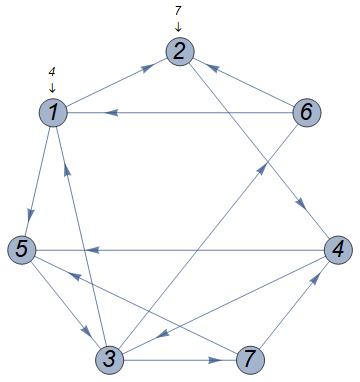
\includegraphics[scale=0.7]{grs/g1.png}\\
%     Рисунок 1 --- Пример рассматриваемого графа $G$
% \end{center}
% \begin{center}
%     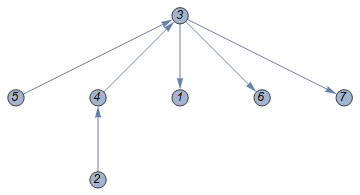
\includegraphics[]{grs/g2.png}\\
%     Рисунок 2 --- Пример опоры графa $G$
% \end{center}


% \begin{center}
%     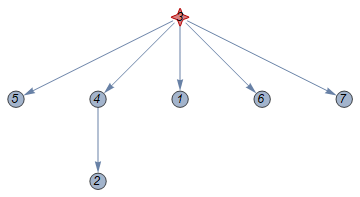
\includegraphics[]{grs/g3.png}\\
%     Рисунок 3 --- Пример корневого дерева $(T^*,r)$
% \end{center}
% Теперь пара $(T,r)$ образует корневое дерево. На рисунке 3 показан пример такого корневого дерева, корень помечен как звезда.

% Для представления корневого дерева в памяти воспользуемся корневыми структурами. 
% \begin{center}
%     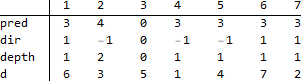
\includegraphics[]{grs/t1.png}\\
%     Таблица 1 --- Пример корневых структур для дерева $T$
% \end{center}

% В таблице 1 приведены корневые структуры для рассматриваемого дерева. Здесь $pred$ --- список предков, в котором в ячейке, соответствующей номеру узла $v\in I^T$ записан номер предыдущего узла из цепи $C(r,v)$, для всех $v\in I^T\setminus \{r\}$. У корневого узла предок не определен, так что $pred[r]=0$. $dir$ --- список направлений, $dir[v]=1$ если $(pred[v],v)\in U^T$ и $-1$, если $(v,pred[v])\in U^T$, $dir[r]::=0$.

% Для описания дерева $T$ приведенных структур достаточно, однако для эффективной работы с ними необходимо добавить 2 вспомогательных структуры: $depth$ и $d$. $depth$ --- список глубин, для каждого узла хранит расстояние от него до корня. $d$ --- список династического обхода дерева, или его топологическая сортировка.

% Алгоритм построения остова и корневых структур приведен в модуле $buildTree$ Листинга А1.

% Для вычисления характеристических векторов дуг используется алгоритм нахождения наименьшего общего предка (least common ancestor, lca). Утверждается, что при добавлении дуги к корневому дереву образуется ровно 1 цикл, и этот цикл состоит из добавленной дуги $(u,v)\in U^T$, $C(u,lca(u,v))$ и $C(v,lca(u,v))$. Таким образом вычисление $\delta_{uv}$ сводится к вычислению $lca(u,v)$ и подъему от каждого из концов дуги к их $lca$. Т.к. предварительно построен список высот, то нахождение $lca$ может быть выполнено за $O(|I|)$ операций подъема, и сложность вычисления всех характеристических векторов составляет $O(|I|*(|U|-|I|))$ операций, а в силу разреженности графа $G$ имеем $|U|\leq c|I|$, где $c<<|I|$ --- некоторая константа, и тогда $O(|I|*(|U|-|I|))=O(|I|^2)$.

% Вычисление определителей циклов происходит по приведенным выше формулам и использует алгоритмы перемножения разреженных матриц.

% Рассмотрим теперь случай графа $G=(I,U)$ с переменным внешним потоком. В таком случае опора представляет собой лес деревьев. Однако задача построения такой опоры может быть сведена к предыдущей. Для этого добавим к графу $G$ фиктивный узел $i'$ и дуги для каждого узла с переменным внешним потоком в (из) вершину $i'$. Внешний поток в узле $i'$ постоянный и может быть найден из глобального уравнения баланса и уравнения баланса для узла $i'$. Таким образом граф $G$ преобразован в граф $G'$ с постоянным внешним потоком и для него можно построить опору как было рассмотрено ранее. Если теперь из полученной опоры удалить фиктивный узел, то дерево распадется на лес, который и будет опорой графа $G$.

% Заметим, что для удобства работы фиктивную вершину можно и не удалять, тогда характеристики вершин с переменным внешним потоком будут совпадать с характеристиками соответствующих фиктивных дуг, как показано в листинге B1-B2.
% \newpage
% \begin{center}
%     \textbf{Заключение}
% \end{center}

% В ходе выполнения данной работы рассмотрена разреженная недоопределенная система линейных алгебраических уравнений и соответствующий ей мультиграф $G=(I, U)$. Для этих СЛАУ и мультиграфа приведены необходимые теоремы и определения и рассмотрены соответствующие теоретические свойства рассматриваемого мультиграфа. После этого введена соответствующая математическая модель и сформулирована задача о расположении специальных программируемых устройств (сенсоров) в узлах мультиграфа. Для сформулированной задачи приведены алгоритмические и структурные свойства построения оптимального решения. В итоге рассматриваемая задача сводится к решению одной из уже известных задач.


% В системе компьютерной алгебры Wolfram Mathematica создан пользовательский пакет "FlowSolwer.m"\ , в котором реализованы программные модули и базовые функции для построения и работы с опорой мультиграфа (мультисети) для случая однородного потока (смотри Листинг А1) и для случая переменного внешнего потока (смотри Листинг B1). Для описания опоры мультиграфа используются расширенные корневые структуры описания деревьев, включающие базовые структуры, список династического обхода и список глубин для уменьшения асимптотической сложности алгоритмов работы с ними. В пакете также реализованы модули для построения частного решения неоднородной системы уравнений баланса, общего решения однородной системы уравнений баланса, общего решения неоднородной системы уравнений баланса, построения характеристических векторов для дополнительной системы, и вычисления детерминантов циклов, а также построения общего решения для системы вида (\ref{f1})-(\ref{f2}). Все перечисленные алгоритмы реализованы для случая однородного потока. Их работа продемонстрирована в Листинге А2 на примере графа, описанного в файле "gr.txt"\,, содержание которого можно найти в Листинге А3.
\newpage
\begin{center}
    \textbf{Список Литературы}
\end{center}
1. L. A. Pilipchuk, Y. V. Malakhouskaya, D. R. Kincaid, and M. Lai, East-West J. of Mathematics 4, No 2, (2002), 191-201.\\
\\
2. Пилипчук Л. А. Линейные неоднородные задачи потокового программирования: учеб.-метод. пособие / Л. А. Пилипчук. - Минск: БГУ, 2009. - 222 с.\\
\\
3. L. A. Pilipchuk, A. S. Pilipchuk, Y. H. Pesheva, International Journal of Pure and Applied Mathematics (IJPAM) 54, No 2, (2009), 193-205.\\
\\
4. I. V. Romanovski, L. A. Pilipchuk, Computing 76, (2006), 353-357.\\
\\
5. L. Bianco, G. Confessore, M. Gentili, Combinatorial Aspects of the Sensor Location Problem. Annals of Operation Research 144, 1, (2006), 201-234.\\
6. Пилипчук, Л. А. Разреженные недоопределенные системы линейных алгебраических уравнений / Л. А. Пилипчук. – Минск : БГУ, 2012. – 260 с.
\end{document}
% \begin{center}
% \includegraphics[scale=0.8]{whatISee.png}
% \end{center}%